%!TEX root = thesis.tex
\chapter{Data, Preprocessing and Features}\label{ch:preprocessing}

\begin{wrapfigure}{r}{7cm}
  \vspace{-35pt}
  \begin{center}
    \newcommand*{\xMin}{0}%
\newcommand*{\xMax}{6}%
\newcommand*{\yMin}{0}%
\newcommand*{\yMax}{6}%
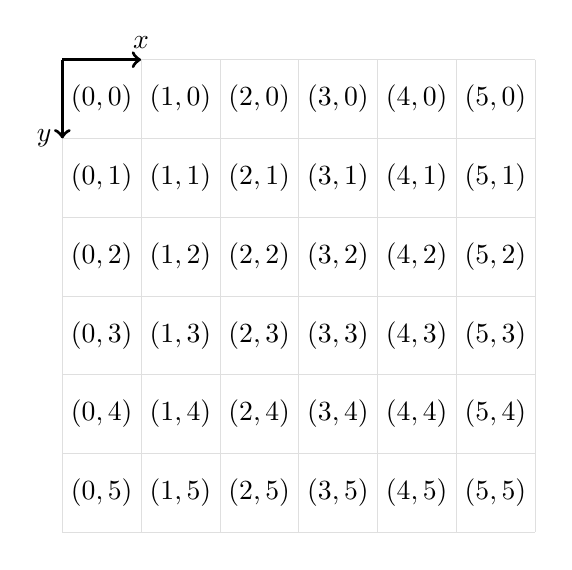
\begin{tikzpicture}[y=-1cm]
    \foreach \i in {\xMin,...,\xMax} {
        \draw [very thin,gray!25] (\i,\yMin) -- (\i,\yMax)  node [below] at (\i,\yMin) {};
    }
    \foreach \i in {\yMin,...,\yMax} {
        \draw [very thin,gray!25] (\xMin,\i) -- (\xMax,\i) node [left] at (\xMin,\i) {};
    }
    \draw[->, very thick] (0,0) -- (1,0) node[above] {$x$};
    \draw[->, very thick] (0,0) -- (0,1) node[left] {$y$};
    \foreach \x in {\xMin,...,5} {
        \foreach \y in {\yMin,...,5} {
            \node at ({\x+0.5},{\y+0.5}) {$(\x, \y)$};
        }
    }
\end{tikzpicture}
  \end{center}
  \vspace{-20pt}
  \caption{HTML5 canvas plane. Each step is one pixel. There cannot be non-integer
           coordinates.}
  \label{fig:canvas-plane}
  \vspace{-10pt}
\end{wrapfigure}

The data that was used for all experiments was collected with
\href{http://write-math.com}{write-math.com}, a website designed solely for
this purpose. This website makes use of HTML5 canvas elements. Those elements
can be used to track fingers or a mouse coursor touching the canvas, moving
and lifting. The origin is at the upper left corner and get bigger to the right
($x$-coordinate) and to the bottom ($y$-coordinate).

The data is stored and shared in JSON format. Each handdrawing is stored as a
list of lines, where each line consists of tuples $(x(t), y(t), t)$, where $x$
and $y$ are canvas coordinates and $t$ is a timestamp in seconds. This timestamp
gives the time in milliseconds from 1970.

The time resolution between points as well as the resolution of the image
depends on the device that was used. However, most symbols have a time
resolution of about $\SI{20}{\milli\second}$ and are within a bounding box of a
$250 \text{px} \times 250 \text{px}$ square.

\section{Preprocessing}\label{sec:preprocessing}
\subsection{Normalization: Scaling, shifting and resampling}
In \cite{Kirsch} the datapoints were scaled to fit into a unit square while
keeping their aspect ratio. Afterwards, the points were shifted to
the $(0, 1) \times (0, 1)$ unit square. The algorithm is given in pseudocode on
\cpageref{alg:scale-and-shift}. It was shown in \cite{Kirsch,Huang09} that
this kind of preprocessing boosts classification accuracy significantly.

Another method to normalize data is resampling, sometimes also called
stroke length normalization.
\cite{Guyon91} resampled characters and digits to 81 points each, where different
lines were also connected by \enquote{pen-up} segments. They resampled to get
points regulary spaced in arc length, not in time. \cite{ICASSP-94} also
resampled data to get points regulary spaced in arc length, but they encoded
speed as an extra feature.

\subsection{Noise reduction}
The following list of noise reduction methods was created by \cite{Tappert90}
and is still up-to-date.\nopagebreak
\begin{itemize}
    \item \textbf{Smoothing} can be done in multiple ways. An approach that was
          used quite often is applying a weighted average
          \cite{Groner66,Division87,Arakaw83}. \cref{alg:weighted-average-smoothing}
          describes in pseudocode how to implement weighted average smoothing.
    \item \textbf{Wild-point detection} and deletion or replacement of 
          wild points with the average of neighboring points\cite{Division87},
    \item \textbf{Filtering} is the process of removing points by some criteria.
          Those criteria include:
          \begin{itemize}
              \item Duplicate points,
              \item Enforcing a minimal distance between consecutive 
                    points\cite{Tappert90}.
              \item Enforcing a minimal change in direction\cite{Tappert90}.
          \end{itemize}
          An idea that seemingly nobody has tried before is applying the
          Douglas-Peucker algorithm for filtering dots.
    \item \textbf{Dehooking} [TODO: Image of hook]
    \item \textbf{Dot reduction} reduces dots to single points. Sometimes
          multiple points get recorded although the user wanted to make only
          a single point, e.g. for one of the following symbols:
          $\cdot$, ., $\dots$, $\vdots$, $\ddots$, i, ä, ö, ü.
          This can be detected by calculating
          the maximum distance $d$ two points in a stroke have. If $d$ is
          smaller than a threshold $\theta$, then it is a single point.
          In that case all points of the line get reduced to a single dot.
          This dot could be the center of mass of all points in the stroke.
    \item \textbf{Stroke connection} might be used if the distance between
          pen-up and pen-down is below a threshold.
    \item \textbf{Deskewing} corrects character slant.
    \item \textbf{Baseline drift correction} moves words to be on a baseline.
\end{itemize}

Wild points are points that appear within a sequence of points of a stroke. They
that were not caused by the pen, but by a hardware error. They are characterized
by a very high velocity and sharp angles.

\section{Features}\label{sec:features}
A number of different features have been suggested so far for on-line handwriting
recognition. They can be grouped into local features and global features.
Local features apply to a given point on the drawing plane and sometimes even
only to point on the drawn curve whereas global features apply to a complete
line or even the complete image.

\subsection{Local features}
\begin{itemize}
    \item Coordinates of the current point\cite{Guyon91}
    \item Speed\cite{Huang09,ICASSP-94}
    \item Binary pen pressure\cite{Kosmala98,Kosmala11,ICASSP-94}
    \item Direction\cite{Manke95,Huang06}
    \item Curvature\cite{Groner66,Manke95,ICASSP-94,Guyon91}
    \item Bitmap-environment\cite{Manke95}
    \item Hat-Feature\cite{ICASSP-94,Manke00}
\end{itemize}

\cite{Kosmala98,Kosmala11} suggest that speed is a bad feature, because it \enquote{highly inconsistent}.

The \textbf{direction} $\text{dir}$ at the point $i$ can be described by the vector 
$(\cos \theta(i), \sin \theta(i))$ as described in \cite{Guyon91}.

\begin{align}
    \cos \theta(i) &= \frac{\Delta x^{(i)}}{\Delta s^{(i)}}\\
    \sin \theta(i) &= \frac{\Delta y^{(i)}}{\Delta s^{(i)}}
\end{align}

where

\begin{align}
    \Delta x (i) &= x^{(i+1)} - x^{(i-1)}\\
    \Delta y (i) &= y^{(i+1)} - x^{(i-1)}\\
    \Delta s (i) &= \sqrt{\Delta (x^{(i)})^2 + \Delta y (y^{(i)})^2}
\end{align}

The \textbf{curvature} $\phi$ of the point $i$ can be described by the
angle of the two neighboring points:

% TODO!
% \begin{align}
%     \text{cur}(i) &= \text{dir}(i-1)
% \end{align}

\subsection{Global features}
\begin{itemize}
    \item Re-curvature\cite{Huang06} (TODO: Explain (all))
    \item Center point\cite{Huang06}
    \item Stroke length\cite{Huang06}
    \item Number of strokes\cite{Huang09}
    \item Pseudo-Zernike Features (TODO: Really global? What is it?)\cite{Khotanzad}
    \item Shadow Code Features\cite{Khotanzad}
\end{itemize}